\documentclass[a4paper, 12pt]{article}

% Layout
\usepackage{geometry}
\geometry{left=16mm}
\geometry{right=10mm}
\geometry{top=1cm}
\geometry{bottom=1cm}

% Paragraph
\usepackage{indentfirst}
\setlength{\parindent}{0.75cm}
\linespread{1.25}

% Font
\usepackage{fontspec}
\usepackage[english,russian]{babel}
\usepackage{microtype}

% \usepackage{polyglossia}
% \setmainlanguage{russian}
% \setotherlanguage{english}

% \newfontfamily{\cyrillicfont}{Droid Serif}
% \newfontfamily{\cyrillicfontrm}{Droid Serif}
% \newfontfamily{\cyrillicfontsf}{Droid Sans}
% \newfontfamily{\cyrillicfonttt}{DejaVu Sans Mono}

\setmainfont{Times New Roman}
\setromanfont{Times New Roman}
\setsansfont{Droid Sans}
\setmonofont{DejaVu Sans Mono}

% Hyphens
\usepackage{hyphenat}
\usepackage{ucharclasses}
\setTransitionsForLatin{\begingroup\hyphenrules{english}}{\endgroup}

% Formulas
\usepackage{amssymb, amsfonts, amsmath}

% Miscellaneous
\usepackage{enumerate}
\usepackage{float}
\usepackage{multirow}

% Hyper references
\usepackage{hyperref}
\hypersetup{
    hidelinks,
    allcolors=black
}

% Images
\usepackage{graphicx}
\graphicspath{ {images/} }

%Including title
\usepackage{pdfpages}

% Figures
\usepackage{chngcntr}
\counterwithin{figure}{section}
\usepackage{subcaption}
\renewcommand\thesubfigure{\asbuk{subfigure})}
\captionsetup[subfigure]{labelformat=simple, labelsep=space}

% Counters
\usepackage[figure,table,page]{totalcount}
\usepackage{totcount}

% Code listings
\usepackage{listings}
\usepackage{xcolor}

\definecolor{codegreen}{rgb}{0,0.6,0}
\definecolor{codepurple}{rgb}{0.58,0,0.82}
\lstdefinestyle{codestyle}{
    commentstyle=\color{codegreen},
    keywordstyle=\color{magenta},
    stringstyle=\color{codepurple},
    basicstyle=\ttfamily\footnotesize,
    breakatwhitespace=false,
    breaklines=true,
    captionpos=b,
    keepspaces=true,
    showspaces=false,
    showstringspaces=false,
    showtabs=false,
    tabsize=2
}

\bibliographystyle{gost780s}



\newtotcounter{citenum} %From the package documentation
\def\oldbibitem{}
\let\oldbibitem=\bibitem
\def\bibitem{\stepcounter{citenum}\oldbibitem}

\begin{document}
\includepdf[pages={1}]
{title.pdf}

\tableofcontents
\newpage

\section{Введение}
Обеспечение кибербезопасности на сегодняшний день является одной из наиболее актуальных проблем.
Она давно поднялась с уровня частных лиц до уровня крупных организаций. Возникла необходимость
создания интеллектуальных систем, способных автоматизировать процесс анализа степени защищенности
программного обеспечения этих организаций. Применение интеллектуальных систем в защите
информационного пространства охватывает очень широкий набор направлений.
В настоящий момент такие системы используются в следующих сферах \cite{spheres}:

\begin{itemize}
\item
Биометрические системы идентификации на основе интеллектуальных
систем активно применяются в банковской сфере.
\item
Системы обнаружения,
предупреждения, реагирования на инциденты и ликвидацию последствий компьютерных атак.
\item
Интеллектуальные системы антивирусной защиты, применяются для контроля каналов проникновения вирусов,
для защиты от вирусов, ``червей'', нежелательных программ, для оповещения при ``заражении'', для ``лечения''
от вирусов.
\end{itemize}

Вторые так же могут служить основанием для когнитивных подходов к оценке кибербезопасности \cite{kognmodels}.

Некоторые из проектов интеллектуальных систем по обеспечению компьютерной безопасности
на данный момент существуют только в концептуальном виде \cite{concept}, но есть и реализованные,
основанные на онтологиях и технологии интеллектуальных многоагентных систем \cite{multigent}.

Цель данной работы --- рассмотреть применение интеллектуальных систем для обеспечения компьютерной
безопасности различных организаций и общественных структур и изучить самые популярные подходы
к построению такого рода систем.

\section{Борьба с киберугрозами в энергетической сфере}
Одна из сфер, где наиболее востребованы интеллектуальные системы для поиска информационных угроз
является отрасль энергетики. Цифровизация ее объектов может вызвать возникновение киберугроз,
связанных с внедрением новых решений, применением новых безнес-моделей, сопровождающихся отсутствием
или недостаточностью информации для оперативного принятия решений по обеспечению безопасности объекта.
Требования, предъявляемые к таким системам описаны в работе \cite{reqs}.

Построение ИС, ответственной за данную задачу, происходит по схеме, представленной
в работах \cite{scheme, ontoling}.
Общая структура такой системы включает три компонента:
\begin{itemize}
\item
Экспертную систему (ЭС) -- продукционная ЭС, предназначенную для выявления типовых уязвимостей,
угроз и векторов атак информационно-технологической системы объекта;
\item
Блок байесовских сетей доверия, ответственный за моделирование экстремальных ситуаций, вызванных нарушением
кибербезопасности, определения вероятности наступления последствий;
\item
Блок оценки рисков наступления экстремальной ситуации и последствий от реализации киберугроз
\end{itemize}

Разработка интеллектуальной системы основана на методике анализа угроз и оценки рисков нарушения
информационной безопасности энергетических комплексов \cite{methods}. Основные задачи, которые решает
данная система: анализ киберугроз, моделирование сценариев, и оценивание рисков.
Для ее реализации была придумана совокупность систем онтологий, отвечающих за отдельные аспекты проблемы.
Схема этой системы представлена на рис. \ref{dio}.

\begin{figure}[h]
    \center{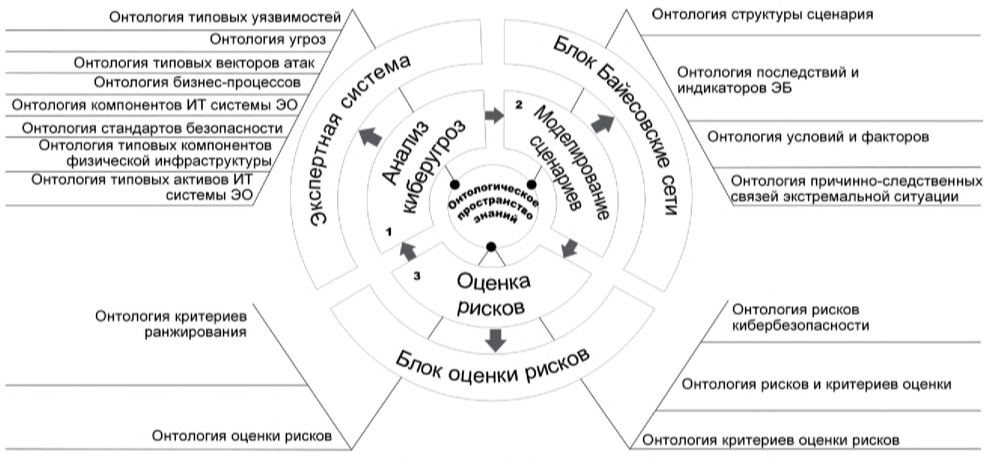
\includegraphics[width=1\linewidth]{scheme}}
    \caption{Строение системы онтологий}
    \label{dio}
\end{figure}

Из данной схемы ясно, что для каждой из основных предметных областей создается набор онтологий, связанных
между собой. В разделе, связанным с анализом киберугроз, онтологический инжениринг позволяет систематизировать
информацию об различных информационно-технологических характеристиках конкретных энергетических объектов
и создать базу знаний их уязвимостей и угроз. В последствии она послужит компонентом для алгоритма проведения
аудита безопасности предприятий и моделировании сценариев возможных экстремальных ситуаций.

За сценарное планирование отвечает байесовская сеть доверия. Сами же сценарии включают в себя следующие данные:
факторы, влияющие на возникновение экстремальных ситуаций, уязвимостей ИТС объекта, природу самой угрозы,
последствия реализации угрозы. В данном случае онтологический инжениринг применяется для создания онтологии
экстремальных сценариев. Конечным результатом работы данной сети должна стать оценка вероятности наступления
того или иного опасного события. При создании множества сценариев их результаты объединяются в онтологию
последствий. В дальнейшем эта онтология служит базой знаний для оценки рисков.

Финальным этапом обработки информации о киберугрозах является оценивание рисков, полученных на основе базы
знаний с вероятностями различных экстремальных ситуаций. Риск рассматривается как комбинация последствий
произошедшего события и возможности его возникновения. Если при анализе рисков обнаружена уязвимость, это
позволяет определить критические факторы возникновения киберугроз на предприятии.

\section{Интеллектуальные системы и кибербезопасность в транспорте}
\newpage

\section{Использование онтологий в информационных войнах}
Понятие информационной войны подразумевает использование информационных и коммуникационных
технологий для достижения преимуществ по сравнению с потенциальным противником. В данном контексте
информационные структуры рассматриваются как системы, хранящие информацию, обрабатывающие ее и определяющие,
представляет тот или иной пакет угрозу или нет. Для этой цели используется онтологический подход к созданию
интеллектуальной системы, предоставляющей базу знаний для потенциального обучения на ней нейронной сети
или иной самообучающейся системы. В работе \cite{wars} приводится пример онтологии, с помощью которой
можно определить киберугрозу. Структуру такой онтологии можно увидеть на рис. \ref{ont}.

\begin{figure}[h]
    \center{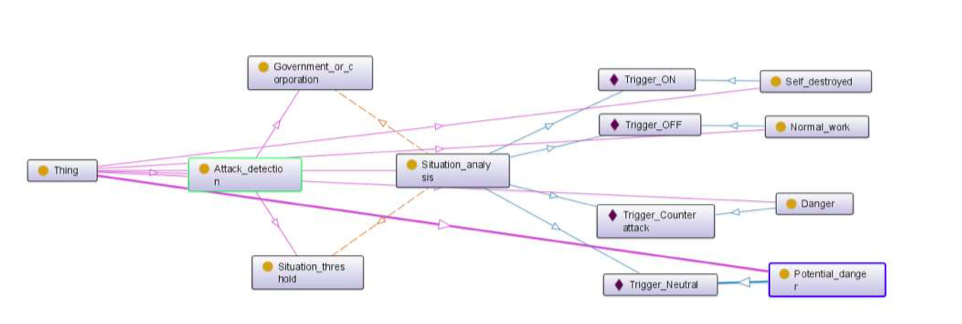
\includegraphics[width=1\linewidth]{ontology}}
    \caption{Структура онтологии для определения угроз}
    \label{ont}
\end{figure}

% TODO Здесь подробнее написать про то, кто каждая компонента представляет (см статью)

\newpage

\section{Заключение}
\newpage

\section{Список литературы}
\medskip

\begin{thebibliography}{}
\bibitem{spheres}
V. Tabakaeva, V. Selifanov, V. An, S. Bularga, and A. Vorozhtsov,
``Intelligent information security management systems'' Trans. Sci. Pap. Novosib. State Tech. Univ., vol. 4,
no. 3–4, pp. 165–176, 2020, doi: 10.17212/2307-6879-2019-3-4-165-176.
\bibitem{kognmodels}
Бурый А.С., Усцелемов В.Н. ``Онтологический подход к формированию когнитивных моделей оценки
кибербезопасности // Информационно-экономические аспекты стандартизации и технического
регулирования.'' 2020. No 3. (55). С. 77-84
\bibitem{concept}
Зыбин Е.Ю., Кривоноженков В.А., Муллин А.Р., Кохан В.В., ``Концепция
интеллектуальной системы обеспечения кибербезопасности бортового оборудования
и систем сверхзвукового пассажирского самолета'', ФГУП ``ГосНИИАС'', 2021
\bibitem{multigent}
И. В. Котенко, ``Интеллектуальные механизмы управления кибербезопасностью'', 2009.
\bibitem{reqs}
Ворожцова Т. Н., ``Онтология как основа для разработки интеллектуальной системы обеспечения
кибербезопасности'' / Т. Н. Ворожцова // Онтология проектирования., 2014, C.69-77
\bibitem{scheme}
D. Gaskova and A. Massel, ``The Technology of Cyber Threat Analysis and Risk Assessment of Cybersecurity
Violation of Critical Infrastructure'' Vopr. kiberbezopasnosti, vol. 2, no. 2(30), pp. 42–49, 2019,
doi: 10.21681/2311-3456-2019-2-42-49.
\bibitem{ontoling}
А. Г. Массель, Д. А. Гаськова, ``Онтологический инжениринг для разработки интеллектуальной системы анализа угроз
и оценки рисков кибербезопасности энергетических объектов'' // Онтология проектирования, pp. 255-238, 2019,
doi: 10.18287/2223-9537-2019-9-2-225-238
\bibitem{methods}
А. Г. Массель, ``Методика анализа угроз и оценки риска нарушения информационно-технологической
безопасности энергетических комплексов'' / А. Г. Массель // XX Байкальской Всероссийской конференции:труды,
т. III. -- Иркутск: ИСЭМ СО РАН, 2015. -- С. 186-195.
\bibitem{}
T. Marzhan, ``Method of development of information security expert system,'' 2019, [Online].
Available: https://proc.ostis.net/wp-content/uploads/2019/10/OSTIS-2019.pdf
\bibitem{wars}
Н. Т. Конференции, “Open Semantic Technologies for Intelligent Systems,” Inf.Tsu.Ru, vol. 7740, no. 3, pp. 145-150, 2019,
[Online]. Available: http://www.inf.tsu.ru/library/Publications/2020/2020-139.PDF.
\end{thebibliography}

\end{document}
